\documentclass[a4paper, 12pt]{article}



%%% Работа с русским языком
\usepackage{cmap}					% поиск в PDF
\usepackage{mathtext} 				% русские буквы в формулах
\usepackage[T2A]{fontenc}			% кодировка
\usepackage[utf8]{inputenc}			% кодировка исходного текста
\usepackage[russian]{babel}	% локализация и переносы

%%% Дополнительная работа с математикой
\usepackage{amsmath,amsfonts,amssymb,amsthm,mathtools} % AMS
\usepackage{icomma} % "Умная" запятая: $0,2$ --- число, $0, 2$ --- перечисление

%% Номера формул
%\mathtoolsset{showonlyrefs=true} % Показывать номера только у тех формул, на которые есть \eqref{} в тексте.

%% Шрифты
\usepackage{euscript}	 % Шрифт Евклид
\usepackage{mathrsfs} % Красивый матшрифт

%% Поля
\usepackage[left=2cm,right=2cm,top=2cm,bottom=2cm,bindingoffset=0cm]{geometry}

%% Русские списки
\usepackage{enumitem}
\makeatletter
\AddEnumerateCounter{\asbuk}{\russian@alph}{щ}
\makeatother

%%% Работа с картинками
\usepackage{graphicx}  % Для вставки рисунков
\graphicspath{{images/}{images2/}}  % папки с картинками
\setlength\fboxsep{3pt} % Отступ рамки \fbox{} от рисунка
\setlength\fboxrule{1pt} % Толщина линий рамки \fbox{}
\usepackage{wrapfig} % Обтекание рисунков и таблиц текстом

%%% Работа с таблицами
\usepackage{array,tabularx,tabulary,booktabs} % Дополнительная работа с таблицами
\usepackage{longtable}  % Длинные таблицы
\usepackage{multirow} % Слияние строк в таблице
\usepackage[table,xcdraw]{xcolor} % Цветные таблицы

%% Красная строка
\setlength{\parindent}{2em}

%% Интервалы
\linespread{1}
\usepackage{multirow}

%% TikZ
\usepackage{tikz}
\usetikzlibrary{graphs,graphs.standard}

%% Верхний колонтитул
\usepackage{fancyhdr}
\pagestyle{fancy}

%% Перенос знаков в формулах (по Львовскому)
\newcommand*{\hm}[1]{#1\nobreak\discretionary{}
	{\hbox{$\mathsurround=0pt #1$}}{}}

%% Мои дополнения
\usepackage{float} %Добавляет возможность работы с командой [H] которая улучшает расположение на странице
\usepackage{gensymb} %Красивые градусы
\usepackage{graphicx}               % Импорт изображений
\usepackage{caption} % Пакет для подписей к рисункам, в частности, для работы caption*
\usepackage{indentfirst} % для отступа красной строки после заголовка

%% TikZ с библиотекой circuits
%% Для рисования электрических схем
\usepackage{tikz}
\usetikzlibrary{circuits}
\usetikzlibrary{circuits.ee}
\usetikzlibrary{circuits.ee.IEC}
\usetikzlibrary{circuits.logic.IEC}

% подключаем hyperref (для ссылок внутри  pdf)
\usepackage[unicode, pdftex]{hyperref}
\tikzset{
  treenode/.style = {shape=rectangle, rounded corners,
                     draw, align=center,
                     top color=white, bottom color=white!20},
  root/.style     = {treenode, font=\ttfamily\normalsize, bottom color=white!20},
  env/.style      = {treenode, font=\ttfamily\normalsize},
  dummy/.style    = {circle,draw}
}
\begin{document}
\newcommand{\HRule}{\rule{\linewidth}{0.7mm}} % Defines a new command for the horizontal lines, change thickness here
	
	\begin{center}
		\large\textbf{Московский Физико-Технический Институт}\\
		\large\textbf{(государственный университет)}
	
		\vfill
		
		\Large Проект для кафедры ЭВМ\\[0.5cm] % Minor heading such as course title
		
		%----------------------------------------------------------------------------------------
		%	TITLE SECTION
		%----------------------------------------------------------------------------------------
		
		\HRule
		\\[0.4cm]
		{ \huge \bfseries Датчик дыхания \newline}
		\\[0.4cm] % Title of your document
		\HRule
		\\[0.5cm]
		
		\ \\
	\textbf{\large Автор:} \\	
	\large Капылов Максим Б01-001

		\vfill
		\hspace*{-0.8 cm}
\includegraphics[width=100 pt]{frkt_logo}\\
		\large Долгопрудный, 2022
	\end{center}

\newpage
\setcounter{page}{2}
\fancyfoot[c]{\thepage}
\fancyhead[L] {Кафедра ЭВМ}
\fancyhead[R]{}
\newpage 

\tableofcontents
\newpage
\section{Введение}
\paragraph{Цель работы:} Обучить нейросеть определять что человек дышит. На вход нейросети будут поданы данные с датчика дыхания и кадры с камеры. После чего нейросеть образует связть между данными и сможет опредять дыхание человека по камере.
\section{Устройство}
\subsection{Функциональная схема}
Схема устройства будет состоять из 4 основных частей.
\linespread{1.3}
\begin{center}
\begin{tikzpicture}
  [
    grow                    = left,
    sibling distance        = 6em,
    level distance          = 10em,
    edge from parent/.style = {draw, -latex},
    every node/.style       = {font=\footnotesize},
    sloped
  ]
  \node [root] {тензодатчик}
    child { node [env] {АЦП}
      child { node [env] {микроконтроллер}
        child { node [env] {ноутбук}
        edge from parent node [below] {} }
      edge from parent node [below] {} }
    edge from parent node [below] {} }; 
    
\end{tikzpicture}
\end{center}
\begin{enumerate}
\item \textbf{Тензодатчик}. Возьмем тензодатчик (рис.1).


	\begin{figure}[h]
		\centering
		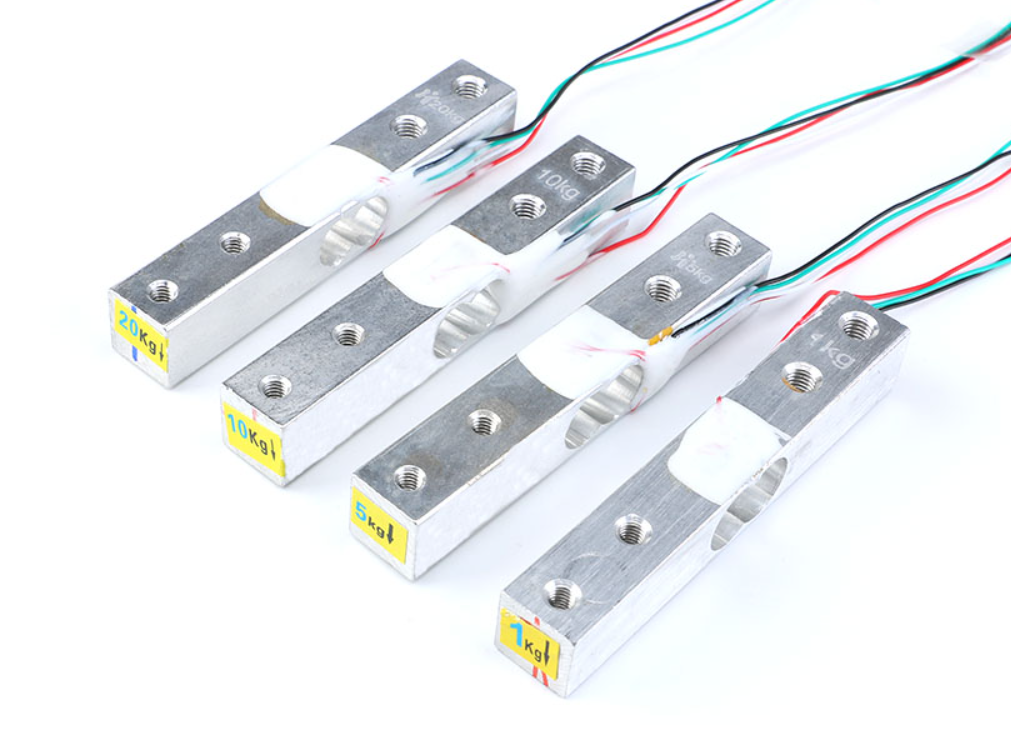
\includegraphics[height= 5cm]{фото_1.png}
		\caption{ТЕНЗОДАТЧИКИ}
	\end{figure}


\item \textbf{АЦП}. В качестве АЦП можно свять модуль HX711. 

\url{https://cdn.sparkfun.com/datasheets/Sensors/ForceFlex/hx711_english.pdf}

\newpage

	\begin{figure}[h]
		\centering
		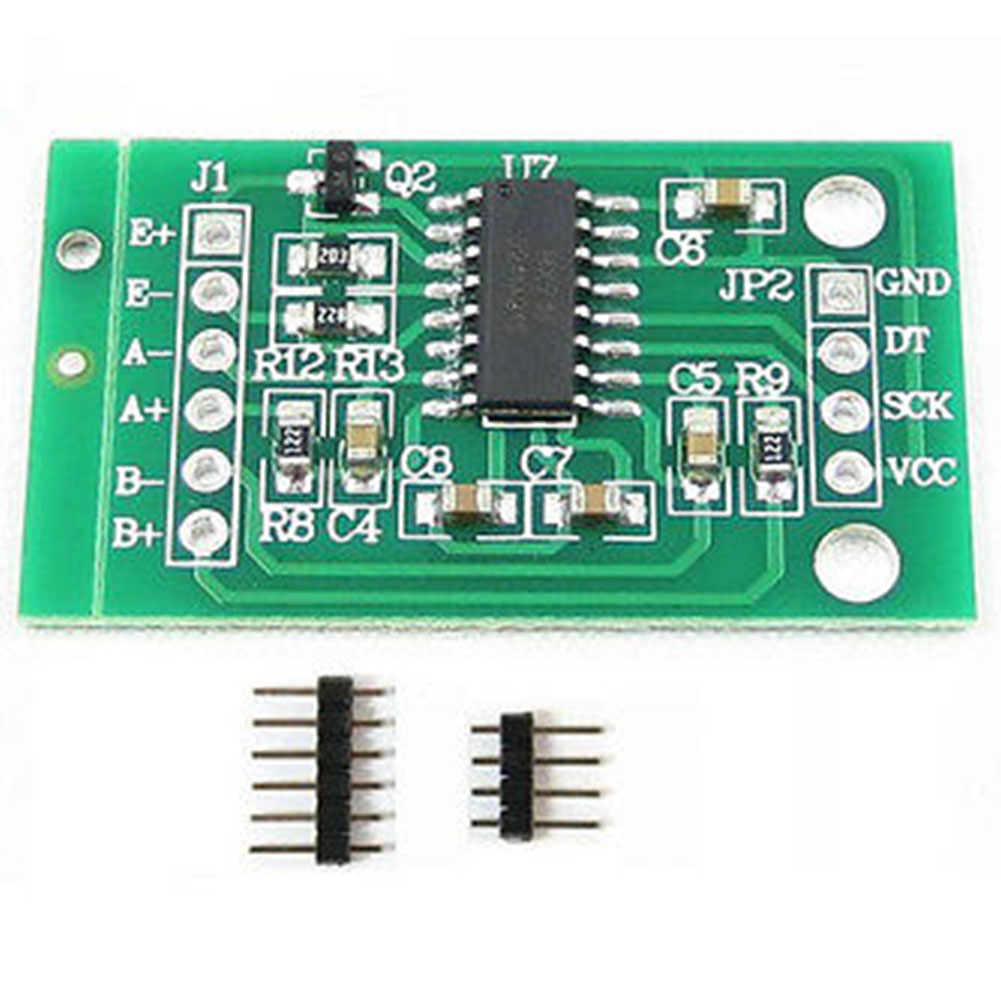
\includegraphics[height= 5cm]{3}
		\caption{АЦП HX711}
	\end{figure}

\item \textbf{Микроконтроллер}. В качестве Микроконтроллер можно взять STM (рис.4)

	\begin{figure}[h]
		\centering
		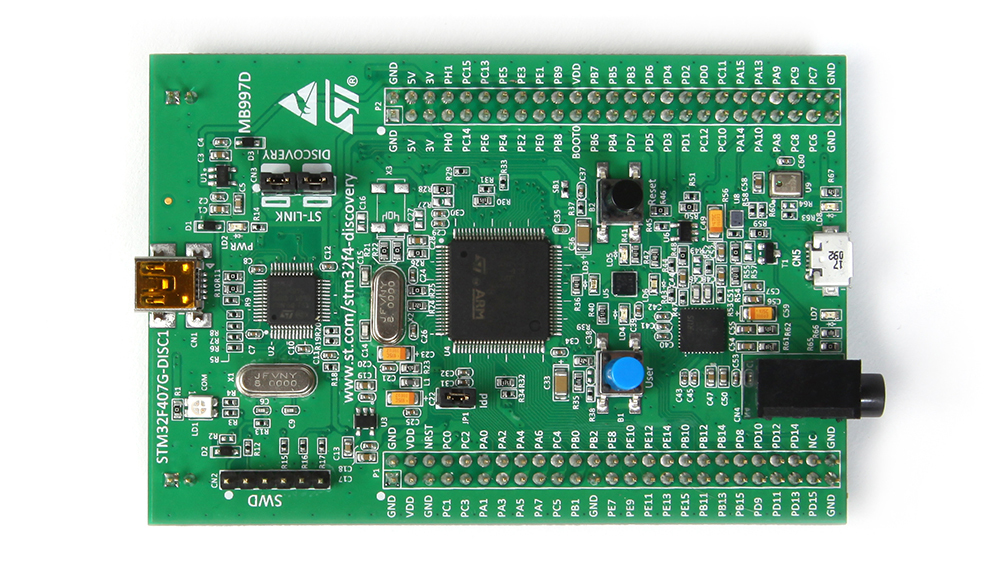
\includegraphics[height= 5cm]{stm}
		\caption{Arduino Nano}
	\end{figure}

\item \textbf{Питание}. Питание схемы будет осуществляться через подключение к ноутбуду через мини usb. 

\section{Крепление}

Крепление датчика к груди с помощью бельевой резинке(рис.6) и застежка Фастекс(рис.7). Чтобы регулировать длину резинки можно использовать пластиковую пряжку (рис.5).

	\begin{figure}[h]
		\centering
		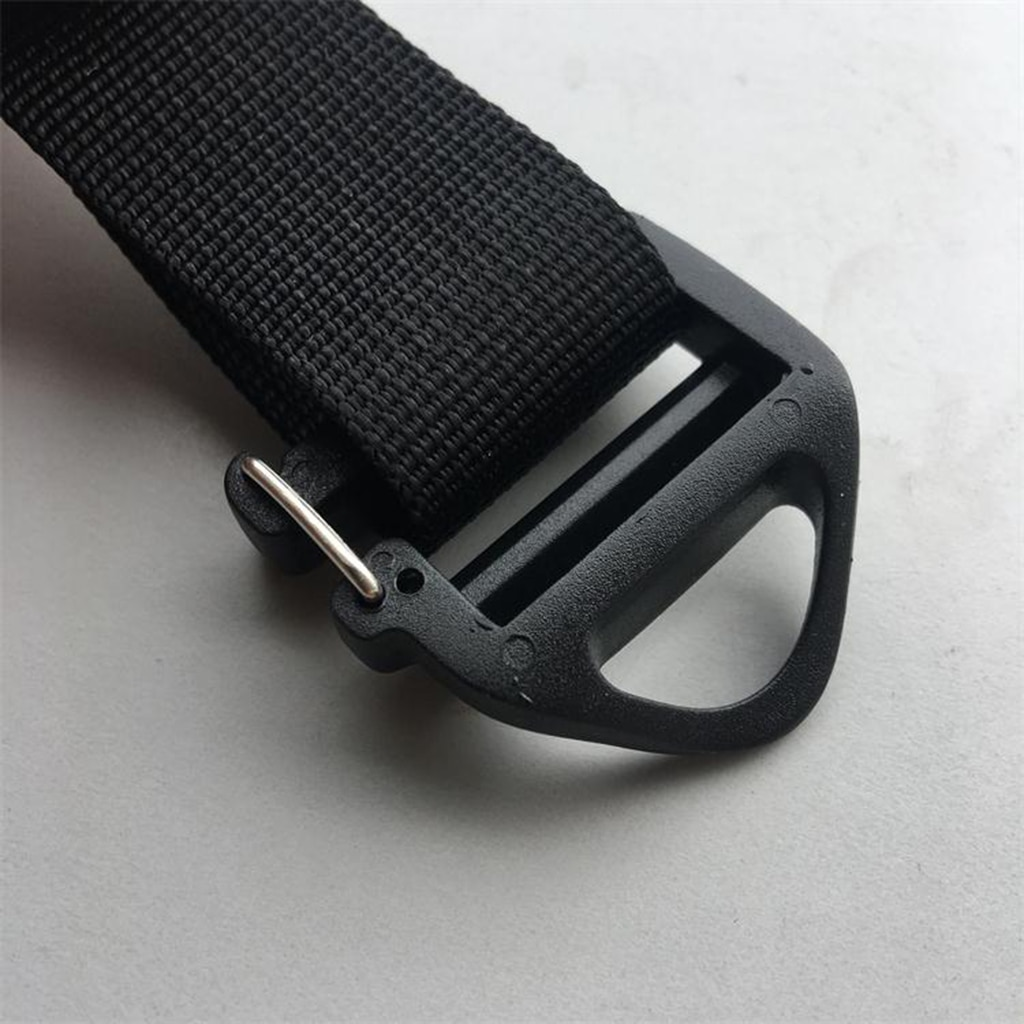
\includegraphics[height= 5cm]{6}
		\caption{пластиковая пряжка}
	\end{figure}

\newpage

\begin{figure}[h]
\begin{center}
\begin{minipage}[h]{0.4\linewidth}
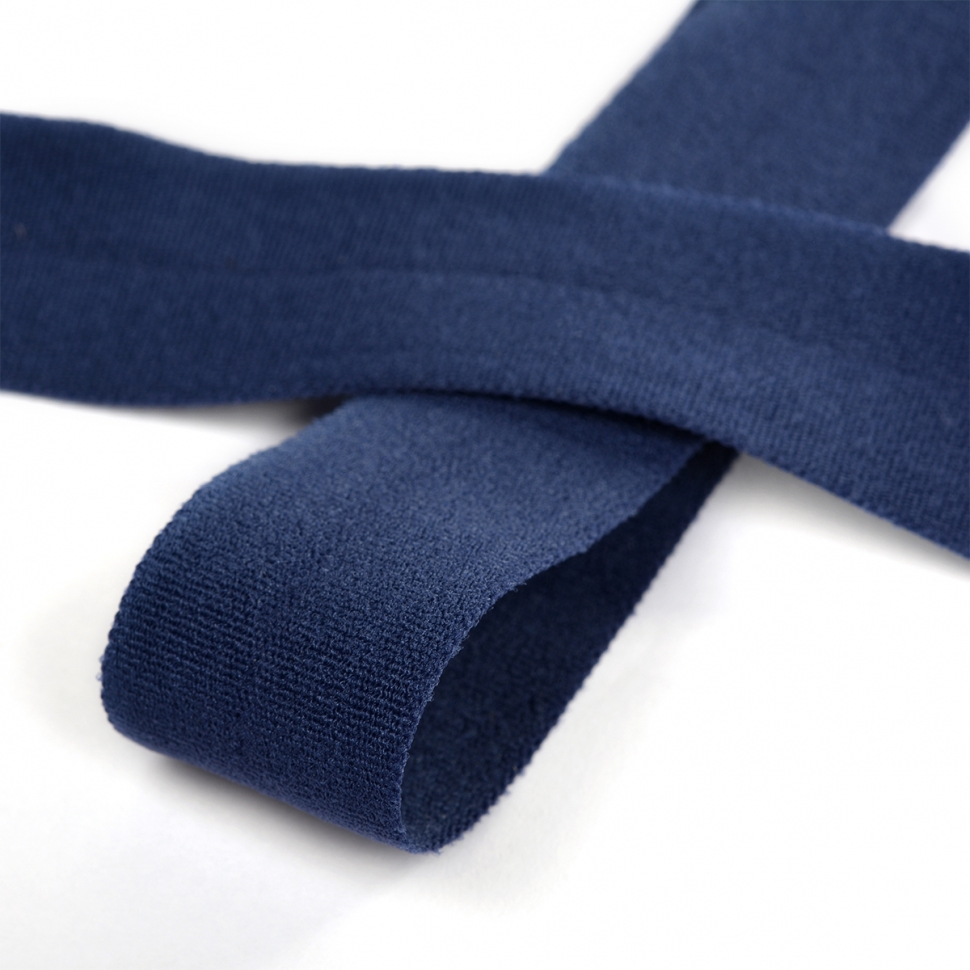
\includegraphics[height= 5cm]{5}
\caption{бельевая резинка} %% подпись к рисунку
\label{ris:experimoriginal} %% метка рисунка для ссылки на него
\end{minipage}
\hfill
\begin{minipage}[h]{0.4\linewidth}
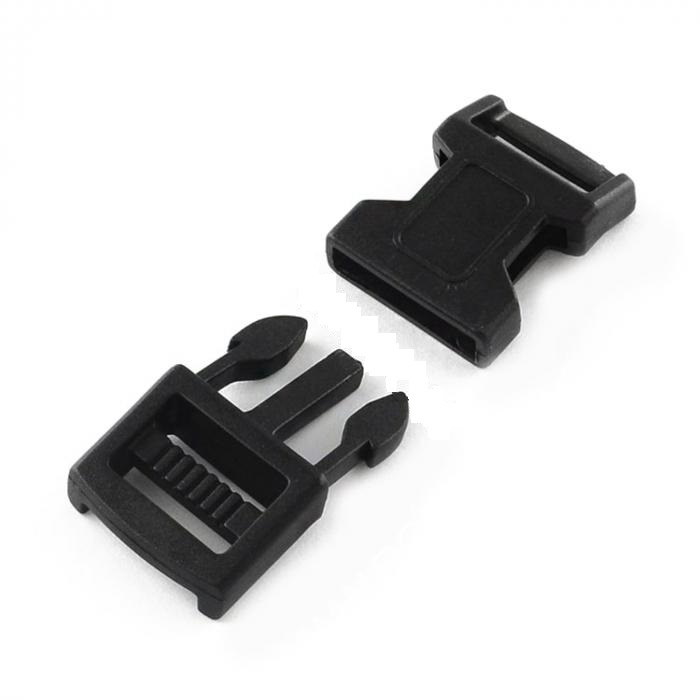
\includegraphics[height= 5cm]{7}
\caption{застежка Фастекс}
\label{ris:experimcoded}
\end{minipage}
\end{center}
\end{figure}
\end{enumerate}
\section{Контсрукция}
\begin{enumerate}

\item В конструкции будут использоватся 2 тензодатчика, основа и 2 плеча. Конструкция будет находится на спине.

	\begin{figure}[h]
		\centering
		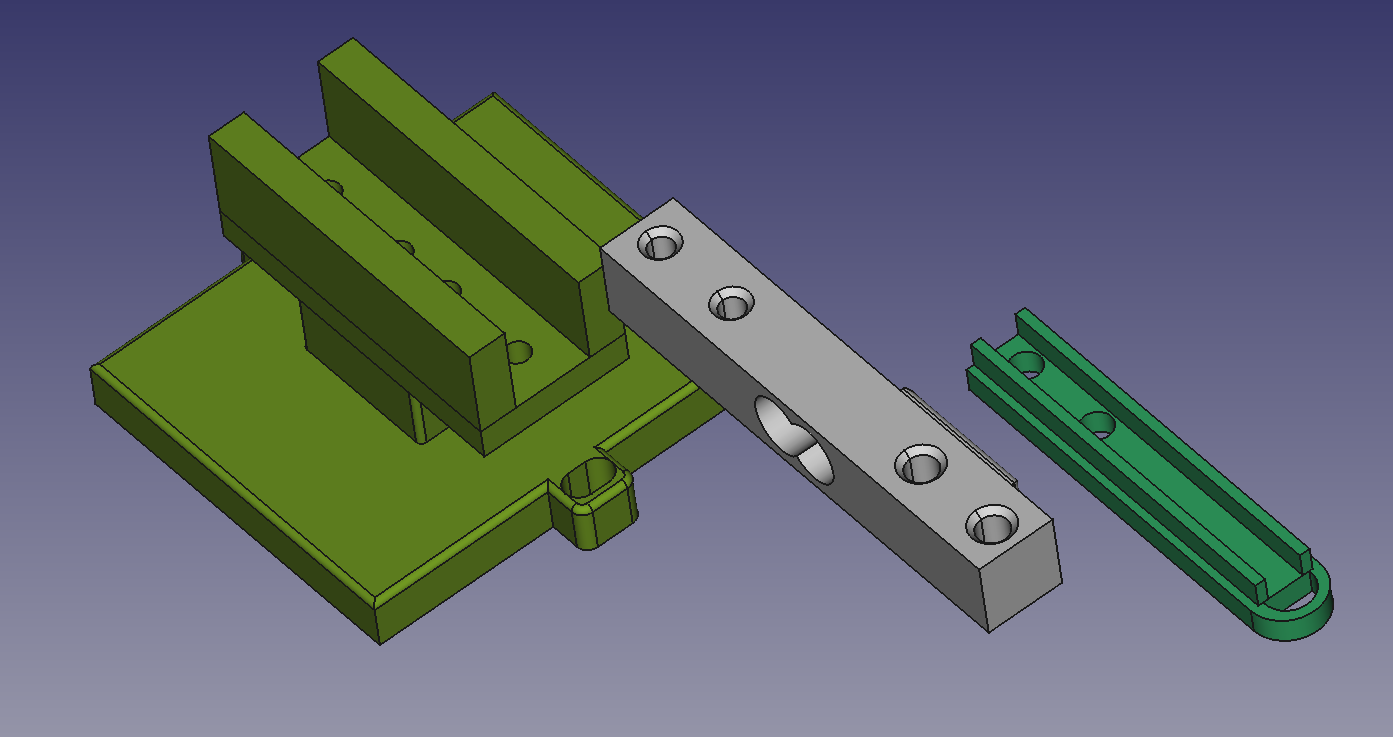
\includegraphics[height= 8cm]{конструкция}
		\caption{конструкция}
	\end{figure}

\end{enumerate} 
\end{document}